\chapter{Night 2: Matrix Operations}

\section*{Overview and Orientation}

\begin{learningobjectives}
\emph{Concepts}
\bi
\item Compute the determinant of a $2\times 2$ matrix
\item Know the relationship between the determinant of a matrix and whether the matrix is invertible
\item Find the inverse of a $2 \times 2$ matrix by hand
\item Use computational tools to find the inverse of an $n \times n$ matrix
\item Design a 2 or 3-dimensional matrix that will scale a vector by given amounts in the $x$, $y$ or $z$ direction
\item Design a 3-dimensional matrix that will translate a 2-D vector by given amounts in $x$ and $y$
\ei
\emph{MATLAB skills}
\bi
\item Represent a set of points in 2-D space (i.e., pairs of $x,y$ values) as column vectors
\item Transform a set of 2-D points (i.e., the outline of a shape) using a matrix to rotate and translate the original
\item Multiply matrices and find their inverses
\item Compute the determinant of a matrix
\ei
\end{learningobjectives}

\subsection{Suggested Approach}
See Night 1 assignment for our general suggested approach to night assignments and a list of linear algebra resources.

\section{Determinant of a Matrix}

The determinant of a square matrix is a property of the matrix which indicates many important things, including whether a matrix is invertible or not. We will see more of this when we see matrix inverses shortly. The determinant of a matrix $\mathbf{G}$ is denoted a few different ways.
\begin{align}
\mbox{det}(\mathbf{G}) &= |\mathbf{G}|
\end{align}


Consider a generic $2\times 2$ matrix $\mathbf{G}$:
\[ \mathbf{G} = \twobytwo{a}{b}{c}{d} \]
The formula for the determinant of a $2\times 2$ matrix is quite straightforward:
\begin{align}
\mbox{det}(\mathbf{G}) &= ad - bc
\end{align}


For example, for the following $2\times 2$ matrix,
\begin{align}
\mbox{det}\left(\twobytwo{1}{2}{3}{4}\right) &= \begin{vmatrix} 1 & 2\\ 3 & 4 \end{vmatrix} \nonumber \\
&=  (1)(4)-(2)(3) =  -2
\end{align}

\begin{prob}\label{ex:det}
Return to the transformation matrices in the day assignment and calculate the determinant for the following:
\begin{enumerate}
    \item The generic $2\times 2$ rotation matrix
    \[ \twobytwo{\cos \theta}{-\sin \theta}{\sin \theta}{\cos \theta} \]
    \item The matrix which reflects over the $y$ axis
    \[ \twobytwo{-1}{0}{0}{1} \]
    \item The matrix which shears in the horizontal direction
    \[ \twobytwo{1}{1}{0}{1} \]
\end{enumerate}
\end{prob}
\begin{sol}
\begin{enumerate}
        \item The determinant is 1. (Recall that $\cos^2\theta + \sin^2\theta = 1$.)
        \item The determinant is -1.
        \item The determinant is 1.
    \end{enumerate}
\end{sol}

 \begin{prob}\label{ex:singular}
 \begin{enumerate}
     \item 
What do the following matrices do? Think about it first, draw some sketches and then test your hypothesis in MATLAB. How much does the area of your basic rectangle change, if at all?
 \begin{enumerate}
 \item \[ \twobytwo{1}{1}{1}{1} \]
 \item \[ \twobytwo{1}{0}{1}{0} \]
% \item \[ \twobytwo{2}{1}{4}{2} \]
% \item \[ \twobytwo{6}{2}{3}{1} \]
 \end{enumerate}
 \item Is it possible to ``undo'' the matrices above? Why or why not?
 \end{enumerate}
 \end{prob}
 \begin{sol}
 \begin{enumerate}
     \item 
 Each of the figures below shows the basic blue rectangle and the orange rectangle, which is the result of applying the transformation.
 \begin{enumerate}
     \item \begin{center}
         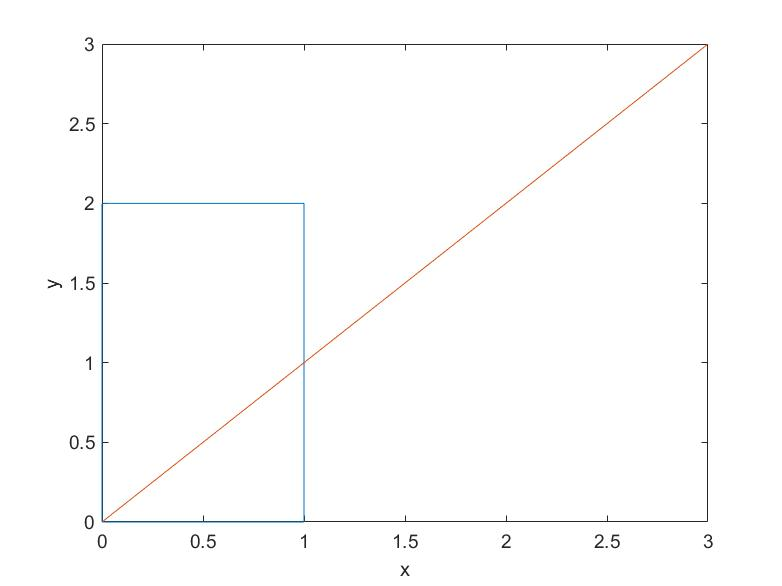
\includegraphics[width=.75\textwidth]{FacesDay2/figs/mat1.jpg}
     \end{center}
         \item \begin{center}
         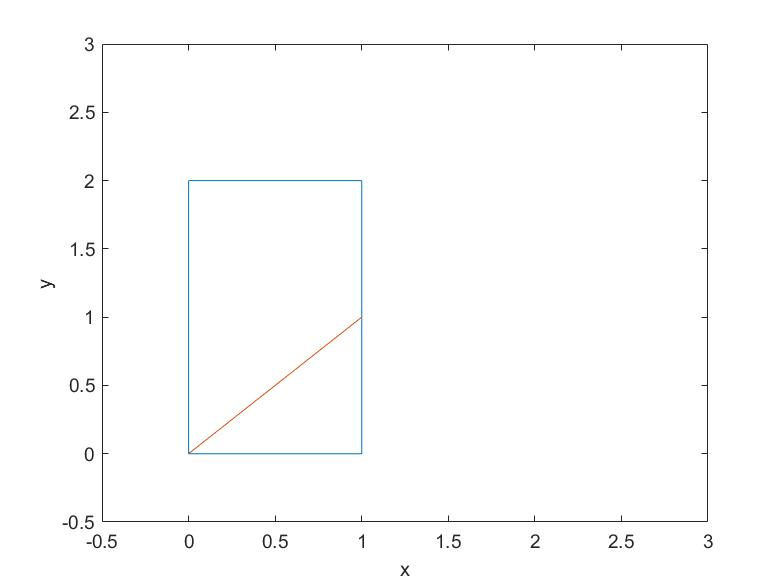
\includegraphics[width=.75\textwidth]{FacesDay2/figs/mat2.jpg}
     \end{center}
%         \item \begin{center}        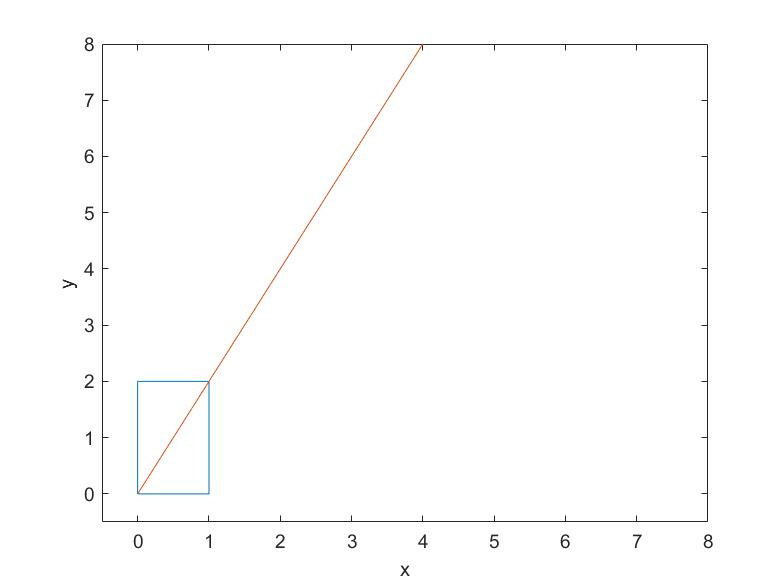
\includegraphics[width=.75\textwidth]{FacesDay2/figs/mat3.jpg}
%     \end{center}
%         \item \begin{center}        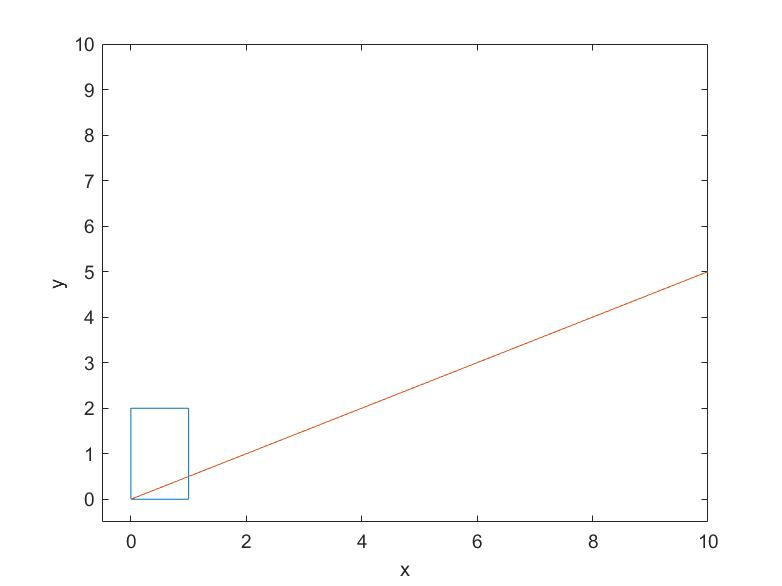
\includegraphics[width=.75\textwidth]{FacesDay2/figs/mat4.jpg}
%     \end{center}
 \end{enumerate}
 \item It is not possible to undo these matrix transformations. Since everything is squished onto the same line, we would not be able to distinguish the original vectors.
 \end{enumerate}
 
 Notice that, in the above matrices, the first row is a constant multiple of the second row. In other words, the matrix looks like $\begin{bmatrix}
 a & b \\ ca & cb
 \end{bmatrix}$ for some constant $c$. If we apply a matrix of this form to a point in 2D space reprsented by the vector $\begin{bmatrix}
 x \\ y
 \end{bmatrix}$, then the result will be $\begin{bmatrix}
 z \\ cz
 \end{bmatrix}$, where $z=ax+by$. In other words, the resulting point will always fall on the line $y=cx$.
 \end{sol}
 
 \begin{prob}
 \begin{enumerate}
     \item What are the determinants of the two matrices from the previous exercise, Exercise~\ref{ex:singular}?
     \item Generalizing from Exercise~\ref{ex:det} and Exercise~\ref{ex:singular}, what's the relationship between the determinant of a matrix and the result of transforming a rectangle by that matrix?
 \end{enumerate}
 \end{prob}

Finding the determinant of an $n\times n$ matrix, where $n>2$, is a bit more computationally intensive. If you want to learn how to do the procedure by hand, check out \href{https://www.khanacademy.org/math/linear-algebra/matrix-transformations/inverse-of-matrices/v/linear-algebra-nxn-determinant}{this Khan Academy video}. For this course, we simply recommend you use the \texttt{det} function in MATLAB. 

%So far, we have mostly talked about rectangles (parallelograms with right angles) as $2\times 4$ matrices. However, we can also think about a $2\times 2$ matrix as representing the same information. For example, the unit rectange could be represented with just the matrix $\mathbf{M}$, where each column is a vector.
%\[ \mathbf{M} = \twobytwo{1}{0}{0}{1} \]
%The two vectors form two sides of a parallelogram (the other two sides are implied).

%%%% SG: I commented out the previous line and modified the text below so it is hopefully clearer.

%% SWM: INSERT PLOT AND COMMENT ABOVE: show rectangle as dot and as two vectors with dashed lines. (or just do this on the board).

%\begin{enumerate}[resume]
%\item Suppose that the columns of a matrix $\A$ are vectors that are not on the same line. Let the columns of this matrix define two sides of a parallelogram (the other two sides, being parallel to these two, are defined automatically).  Show that the magnitude of $det(\A)$ is equal to the area of a parallelogram formed by the column vectors of the matrix $\A$.
%\item What is the determinant of $\A$ if its column vectors are on the same line?
%\end{enumerate}


%\section{Linear Systems of Algebraic Equations: Formulation and Definition [60 mins]}
%
%In previous classes, you've encountered a bunch of exercises where you had to operate on a vector to find another vector:
%\begin{align}
%\A\x = \b,
%\end{align}
%where $\A$ and $\x$ were known, and your job was to find $\b$.  While this is fun, and as you saw above in the rectangle exercise, can be useful, there is another related problem which is easily as important.  It involves the same equation, but now you know $\A$ and $\b$ and need to find the vector $\x$.  As we will discuss here, this problem captures the concept of a Linear System of Algebraic Equations.
%
%One key idea in building models is the step of abstraction: going from some real-world situation to an abstracted model for the system (e.g., a set of differential equations).  There are two important aspects of building such a model: first, deciding what to include or ignore, and second, deciding how to mathematically represent those things you choose to include.
%
%One particularly common kind of mathematical framing is a set of linear algebraic equations, which can be represented by a matrix equation.  You might think ``yeah, but how often are things really linear''?  Well, the answer is ``an awful lot of the time, especially in situations that we care about.''  And when systems do admit to this type of model, linear algebra techniques can be extremely useful for gaining insight.
%
%A general system of $m$ linear algebraic equations in $n$ unknown variables $x_1, x_2, \ldots, x_n$ takes the form
%\begin{eqnarray*}
%a_{11}x_1 + a_{12}x_2 + a_{13}x_3 + \ldots + a_{1n}x_n &=& b_1 \\
%a_{21}x_1 + a_{22}x_2 + a_{23}x_3 + \ldots + a_{2n}x_n &=& b_2 \\
%\ldots &=& \ldots \\
%a_{m1}x_1 + a_{m2}x_2 + a_{m3}x_3 + \ldots + a_{mn}x_n &=& b_m
%\end{eqnarray*}
%where $a_{11}, a_{12}, \ldots, a_{mn}$ are known as coefficients and $b_1, b_2, b_3, \ldots, b_m$ are constants. We can write this using matrices and vectors in the form
%\[ \A \x = \b \]
%where $\A$ is the $m \times n$ {\it coefficient matrix}, $\x$ is the $n \times 1$ unknown vector, and $\b$ is a $m \times 1$ constant vector which is known.
%
%Note that ``linear'' here means linear in terms of the unknown variables, e.g., if x is an unknown there are only terms like $ax$, and no terms like $\sin(x)$, $x^2$, $1/x$, etc.  It is often the case that you might have {\it coefficients} that appear to be non-linear; for example, in solving physics problems, you might have coefficients that depended on trig functions of angles (e.g., $(L \cos \theta) F_x$ is linear in $F_x$ but not linear in $\theta$).  Be careful to be clear about what you're solving for when you decide whether something is linear or non-linear.
%
%\section{Linear Systems of Algebraic Equations: Framing}
%
%Half of the battle is typically getting your system abstracted to the point that it can be thought of as a system of linear equations.   On the following pages are a set of problems.  You don't need to solve these problems -- you just need to formulate them as linear algebra problems.  Please work through these on the board so we can help you!
%
%\clearpage
%
%\subsection{A Mechanical Example}
%
%\begin{marginfigure}
%\includegraphics[width=3.5in]{figs/ClassicSign.jpg}
%\end{marginfigure}
%
%Let's start in a familiar domain from the boat module: statics.   You might recall the sign question from the first module:  the sign is supported on the left by a pin joint which can exert force in both the X and the Y direction $F_X$ and $F_Y$, but cannot sustain any torques, and the sign is supported on the right by a cable which makes an angle of 45 degrees with the sign, and the cable has a tension $T$. We are interested in finding the unknowns $ F_X$, $F_Y$ and $T$. Remembering that the conditions for static equilibrium can be expressed as  $\sum \vec{F} = 0$ and $\sum \vec{\tau} = 0$ write out a linear algebra problem which expresses the static equilibrium conditions in terms of a vector of our unknowns, by considering the sum of forces in the $x$ direction, the sum of forces in the $y$ direction and the torque taken with the pin joint as the axis.
%	
%\clearpage
%\subsection{An Electrical Example}
%
% \begin{marginfigure}
%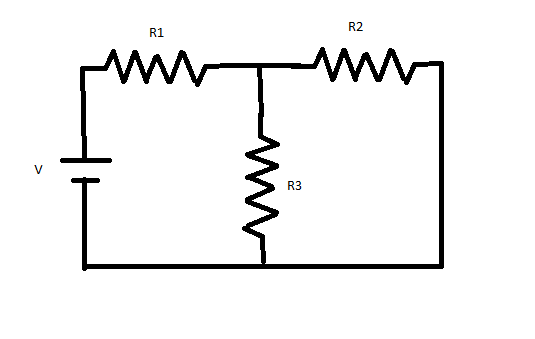
\includegraphics[width=4.5in]{figs/SimpleCircuit.png}
%\end{marginfigure}
%
%Remembering your circuit analysis back from ISIM, recall that Kirkhoff's laws:
%\begin{enumerate}
%\item  Kirkhoff's Voltage Law says that the sum of all the voltage drops around any loop of a circuit must sum to zero.  (Batteries contribute a voltage increase of $V$, resistors contribute a voltage drop of $IR$.)
%\item Kirkhoff's Current Law says that the sum of all current going into and out of any junction of wires in the circuit must be zero.
%\end{enumerate}
%In the circuit at the right, consider that there is a current $I_1$ going through resistor $R_1$, a current $I_2$ going through resistor $R_2$ and a current $I_3$ going through resistor $R_3$.  Find a linear algebra expression for the vector of our three unknown currents.
%
%
%
%\clearpage
%
%
%\subsection{An Investment Example}
%  At your table, discuss the following example.  For each case where you are prompted, decide whether/how you can abstract the system to a mathematical model that can be written as a matrix equation.
%
%Suppose that the following table describes the stock holdings of three of the QEA instructors.
%
%\vspace{0.5cm}
%
%\begin{tabular}{|c|c|c|c|}
%  \hline
%  % after \\: \hline or \cline{col1-col2} \cline{col3-col4} ...
%     & Apple & IBM & General Mills \\
% \hline
%  Jeff & 100 & 100 & 100 \\
%  Rebecca & 100 & 200 & 0 \\
%  John & 50 & 50 & 200 \\
%  \hline
%\end{tabular}
%
%\vspace{0.5cm}
%
%Also suppose that on a given day the value of the Apple, IBM and General Mill's stock are \$100, \$50 and \$20 respectively.
%
%\begin{enumerate}
%\item {\bf Here's your first linear algebra formulation question:} What is the total value of the holdings for each professor on the day in question?  Can you formulate this as a matrix expression?  If so, what is it?
%
%\item Now, suppose that you do not know how many shares of each stock are owned by the instructors. However, you know that the total value of the stocks for each instructor for three consecutive days is as given in the following table
%
%\begin{tabular}{|c|c|c|c|}
%  \hline
%  % after \\: \hline or \cline{col1-col2} \cline{col3-col4} ...
%     & Day 1 & Day 2 & Day 3 \\
% \hline
%  Jeff & \$1500 & \$1600 & \$1400 \\
%  Rebecca & \$2600 & \$2810 & \$2550 \\
%  John & \$950 & \$1020 & \$1000 \\
%  \hline
%
%\end{tabular}
%
%You also know that  the price of each stock on each of the three days was as follows
%
%\begin{tabular}{|c|c|c|c|}
%  \hline
%  % after \\: \hline or \cline{col1-col2} \cline{col3-col4} ...
%     & Day 1 & Day 2 & Day 3 \\
% \hline
%  Apple & \$100 & \$110 & \$100 \\
%  IBM & \$50 & \$50 & \$40 \\
%  General Mills & \$20 & \$22 & \$30 \\
%  \hline
%\end{tabular}
%
%\bf{Now here's the second formulation question:} how many stocks of each company does each professor own?  Can you formulate this as a matrix equation?  If so, what are the matrices/vectors?
%
%\end{enumerate}

%\section{Overview of the homework assignment}

%

\section{Matrix Inverses}

\subsection{Inverse of $2\times 2$ Matrices}

In class you worked with rotation matrices and transformations that were compositions of simpler rotations, and you learned how to invert them. When you multiply a vector by any matrix (not just ones that are associated with simple spatial transformations), you transform the original vector into a new vector. More generally (than rotations), you can \emph{often} undo the linear transformation (just like you did with the rotation matrix). Undoing this linear transformation is a linear transformation itself! Therefore the act of undoing a linear transformation can be formulated with a matrix multiply.

\begin{prob}
Consider the following matrices and vector. (Don't try to interpret these as intuitive geometrical operations; we're just using them to explore the determinant.)  Work out the following problems in MATLAB.
\begin{align}
\mathbf{P} &= \twobytwo{2}{1}{4}{3}\\
\mathbf{Q} &= \twobytwo{\frac{3}{2}}{-\frac12}{-2}{1}\\
\mathbf{u} & = \twobyone{2}{3}
\end{align}
\begin{enumerate}
\item Find $\mathbf{w} = \mathbf{Pu}$.
\item Find $\mathbf{Qw}$. How is this related to $\mathbf{u}$?
\item Find $\mathbf{QP}$. Does the answer look familiar?
\item Find $\mathbf{PQ}$.
\item Find the determinant of $\mathbf{P}$. In MATLAB, you can compute the determinant of any (not just $2\times 2$) matrix using the \texttt{det} function.
\item Find the determinant of $\mathbf{Q}$.
\end{enumerate}
\end{prob}
\begin{sol}
\begin{enumerate}
    \item $$\mathbf{w} = \mathbf{Pu} = \begin{bmatrix}
    7 \\ 17
    \end{bmatrix}$$
    \item $$\mathbf{Qw} = \mathbf{QPu} = \begin{bmatrix}
    2 \\ 3
    \end{bmatrix}$$
    \item $$\mathbf{QP} = \begin{bmatrix}
    1 & 0 \\ 0 & 1
    \end{bmatrix}$$ which is the identity matrix
    \item The determinate of $\mathbf{P}$ is 2.
    \item The determinate of $\mathbf{Q}$ is $\frac12$.
\end{enumerate}
\end{sol}


A matrix $\mathbf{B}$ is said to be the inverse of the matrix $\mathbf{A}$ if, and only if, $\mathbf{BA} = \mathbf{I}$ and $\mathbf{AB} = \mathbf{I}$, where $\mathbf{I}$ is the identity matrix.
For $2 \times 2$ matrices, the inverse (if it exists) is given by the following
\begin{align}
\mathbf{G} &= \twobytwo{a}{b}{c}{d}\\
\mathbf{G}^{-1} &= \frac{1}{ad-bc}\twobytwo{d}{-b}{-c}{a}
\end{align}
The last equation should indicate to you that the inverse of the matrix $\mathbf{G}^{-1}$ is only defined if $ad-bc\neq 0$. Sweet mother of linear algebra, $ad-bc$ is our buddy the determinant. More generally, any square matrix can be inverted if and only if its determinant is non-zero.

Now let's practice calculating inverses, some of their properties, and how we may use them.

\begin{prob}
All matrices $\mathbf{A}$ and $\mathbf{B}$ which have inverses have the following properties
\begin{align}
(\mathbf{AB})^{-1} &= \mathbf{B}^{-1}\mathbf{A}^{-1} \nonumber\\
(\mathbf{A}^{T})^{-1} &= (\mathbf{A}^{-1})^{T} \nonumber
\end{align}
\begin{enumerate}
    \item Using the above properties, please compute the following by hand.
\begin{enumerate}
\item If
\begin{align}
\mathbf{P} &= \twobytwo{2}{1}{4}{3}\\
\mathbf{B} &= \twobytwo{1}{2}{2}{3}\\
\end{align}
find $(\mathbf{PB})^{-1}$. Recall that you already know the inverse of $\mathbf{P}$ from earlier.
\item For $\mathbf{P}$ as defined above, find
\begin{align}
(\mathbf{P}^T)^{-1}
\end{align}
\end{enumerate}

\item Use the inverse formula to calculate the inverses for the first three matrices in Exercise~\ref{ex:det}. Confirm your answers by multiplying the inverse with the original matrix.

\begin{enumerate}
\item By hand, write an equation relating $\mathbf{n}$ and $\mathbf{d}$, using a matrix-vector product.
\item By hand, calculate how many oranges and apples you have.
\item Why do you think this type of problem is often called an inverse problem?
\end{enumerate}
\end{enumerate}
\end{prob}

\begin{sol}
\begin{enumerate}
    \item \begin{enumerate}
        \item $$(\mathbf{PB})^{-1} = \begin{bmatrix}
        -17/2 & 7/2 \\ 5 & -2
        \end{bmatrix}$$
        \item $$(\mathbf{P}^T)^{-1} = \begin{bmatrix}
        3/2 & -2 \\ -1/2 & 1
        \end{bmatrix}$$
    \end{enumerate}
    
    \item    
    
    \[ \left(\twobytwo{\cos \theta}{-\sin \theta}{\sin \theta}{\cos \theta}\right)^{-1} = \twobytwo{\cos\theta}{\sin\theta}{-\sin\theta}{\cos\theta} \]
    
    \[ \left(\twobytwo{-1}{0}{0}{1}\right)^{-1} = \twobytwo{-1}{0}{0}{1} \]
    
    \[ \left(\twobytwo{1}{1}{0}{1}\right)^{-1} = \twobytwo{1}{-1}{0}{1} \]

\end{enumerate}
\end{sol}

Note that solving matrix-vector equations like above can be done without explicitly computing the matrix inverse which is computationally expensive. (A nod to our future friend, left matrix divide or backslash divide.)

\subsection{Inverse of $n\times n$ Matrices}

For higher-dimensional matrices, e.g. $n\times n$ matrices for $n > 2$, the matrix inverse is defined in the same way. Suppose you have an $n\times n$ matrix $\mathbf{A}$ and an $n\times n$ matrix $\mathbf{B}$. Then  $\mathbf{B}$ is the inverse of $\mathbf{A}$ if and only if $\mathbf{BA} = \mathbf{I}$ and $\mathbf{AB} = \mathbf{I}$.  The following are some properties of inverses of matrices

\begin{itemize}
\item Only square matrices are invertible, i.e., only square matrices have inverses.
\item A matrix has an inverse only if its determinant is non-zero.
\end{itemize}

There are a number of different procedures to compute the inverse of higher-dimensional matrices, but we will not be going into the details of their computation here. You can look them up if you are interested, or need to in the future.  In MATLAB, you can compute the inverse of a matrix using the \texttt{inv} function.

\begin{prob}
\begin{enumerate}
\item Consider the example with the fruits that you worked out earlier. Now,  in addition to apples and oranges, suppose you also had an unknown number of pears which each weigh 3 oz, and cost \$3. Additionally, suppose that the total weight of the fruits is 45 oz, and you paid a total of \$21 for the fruit.

    \begin{enumerate}
    \item If possible find the numbers of oranges, apples and pears. If not, please explain why.
    \item Suppose that you additionally know that you have a total of 14 fruits. Can you formulate and solve a matrix-vector equation to find out the numbers of oranges, apples and pears you have?
    \item What is the determinant of the matrix you have set up to solve this?
    \end{enumerate}
\item The fruit vendors bought the pricing algorithm from Uber. Oranges are still \$2, pears are now only \$1.50, and (due to an influx of teachers) apples are now surging at \$1.50 each. Their weights stay the same. You return to the market, and again purchase 14 fruits, which have the same total weight and total cost.
\begin{enumerate}
	\item Can you formulate and solve a matrix-vector equation to find out the numbers of oranges, apples and pears you have?
    \item What is the determinant of the matrix you have set up to solve this?
    \item Debrief at your table about what this means.
 \end{enumerate}
\end{enumerate}
\end{prob}
\begin{sol}
\begin{enumerate}
    \item \begin{enumerate}
        \item It's not possible to find the numbers of oranges, apples, and pears. We have the equation
        $$\begin{bmatrix}
        2 & 1 & 3 \\ 4 & 3 & 3
        \end{bmatrix}\begin{bmatrix}
        n_0 \\ n_a \\ n_p
        \end{bmatrix} = \begin{bmatrix}
        21 \\ 45
        \end{bmatrix},$$
        but we cannot take the inverse of a $2 \times 3$ (non-square) matrix.
        \item Now we have the equation
        $$\begin{bmatrix}
        2 & 1 & 3 \\ 4 & 3 & 3 \\ 1 & 1 & 1
        \end{bmatrix}\begin{bmatrix}
        n_0 \\ n_a \\ n_p
        \end{bmatrix} = \begin{bmatrix}
        21 \\ 45 \\ 14
        \end{bmatrix}.$$
        So by taking the inverse of the $3 \times 3$ matrix we find that $n_0 = 3, n_a = 9$ and $n_p = 2.$
        \item The determinant of the matrix is 2.
    \end{enumerate}
    \item \begin{enumerate}
        \item The equation becomes
        $$\begin{bmatrix}
        2 & \frac32 & \frac32 \\ 4 & 3 & 3 \\ 1 & 1 & 1
        \end{bmatrix}\begin{bmatrix}
        n_0 \\ n_a \\ n_p
        \end{bmatrix} = \begin{bmatrix}
        21 \\ 45 \\ 14
        \end{bmatrix}.$$
        But the matrix is not invertible, so we cannot solve for the number of fruit.
        \item The determinant of the matrix is 0.
        \item
    \end{enumerate}
\end{enumerate}
\end{sol}

\section{Transformation Matrices, Continued}

\subsection{Scaling}

Returning to two dimensions. In the Night 1 assignment, you also learned about scaling matrices. Recall that the scaling matrix $\mathbf{S}$ scales the x-component by $s_1$ and the y-component by $s_2$
\[ \mathbf{S} = \twobytwo{s_1}{0}{0}{s_2}. \]
Let's assume for the moment that $s_1 = 2$ and $s_2 = 1/3$. Working with the rectangles defined in class whose corners have coordinates $(1,2)$, $(1,-2)$, $(-1,2)$, and $(-1,-2)$  complete the following activities:

\begin{prob}
\begin{enumerate}
\item Predict what would happen if you operate on the rectangle with $\mathbf{S}$.
\item Write a MATLAB script to carry out this operation and check your prediction.
\item How does the area of the rectangle change?
\item What matrix should you use to \textit{undo} this scaling? Show that the product of this matrix with the original scaling matrix is the \textit{identity} matrix.
\item Define it in MATLAB and check. Again, this is the \textit{ inverse} matrix and we give it the symbol $\mathbf{S}^{-1}$.
\item In MATLAB, change the value of $s_2$ to 1 and find the product of the new $\mathbf{S}$ and your rectangle.  How does the area of the rectangle change?  Change the value of $s_2$ back to 1/3.
\item Predict what would happen if you operate on the original rectangle with $\mathbf{S} \mathbf{R}$, where $\mathbf{R}$ is the rotation matrix. How about $\mathbf{R} \mathbf{S}$? Implement both of these in MATLAB and check.
\item How would you \textit{ undo} each of these operations ($\mathbf{S} \mathbf{R}$ and $\mathbf{R} \mathbf{S}$)? How is the inverse of the product related to the individual inverses, i.e. what is the relationship between $(\mathbf{S} \mathbf{R})^{-1}$ and $\mathbf{S}^{-1}$ and $\mathbf{R}^{-1}$? What about $(\mathbf{R} \mathbf{S})^{-1}$?
\end{enumerate}
\end{prob}

\begin{sol}
	\begin{enumerate}
		\item The length of the rectangle would double in the x direction and be reduced to 1/3 the length in the y direction.
		\item First we define the corners of the rectangle as the columns in a matrix\\
		{\centering \texttt{>> points=[1 1 -1 -1; 2 -2 -2 2]}}\\
		and we define the scaling matrix\\
		{\centering \texttt{>> S=[2 0; 0 1/3]}.}
		Then we simply multiply them\\
		{\centering \texttt{>> scaledpoint=S*points}.}\\
		Plotting them, here is the original rectangle in blue and the scaled rectangle in orange
		\begin{center}
		    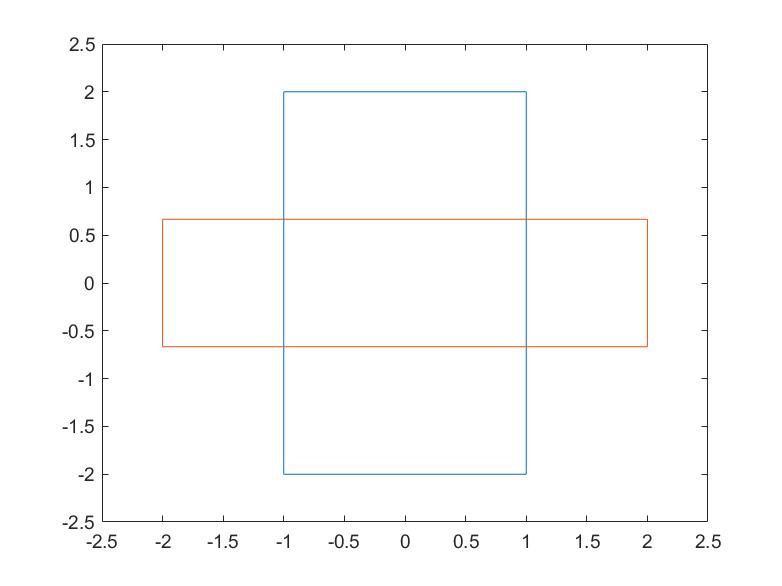
\includegraphics[scale=.5]{FacesNight2/figs/scaledrec.jpg}
		\end{center}
		\item The area is reduced from 8 units$^2$ to 5.33 units$^2$, or 2/3 of the original area.
		\item To undo the process we use the inverse of the $\mathbf{S}$ matrix, or $\mathbf{S}^{-1}$ would be used. \[ \mathbf{S}^{-1} = \twobytwo{0.5}{0}{0}{3}. \]
		You should check that $\mathbf{S}^{-1}\mathbf{S} = \mathbf{SS}^{-1} = \mathbf{I}$.
		\item We define the inverse matrix
		{\centering \texttt{>> Sinv=[0.5 0; 0 3]}}
		and check that \texttt{>> S*Sinv} and \texttt{Sinv*S} both produce the identity matrix.
		\item The area of the rectangle doubles.
		\item When the original rectangle is operated on with $$\mathbf{SR}$$, the resulting image will be a horizontally stretched parallelogram. When the original rectangle is operated on with $\mathbf{RS}$, the resulting image will be the scaled rectangle from the previous exercise only rotated 60 degrees counter-clockwise.
		\item $(\mathbf{SR})^{-1}=\mathbf{R}^{-1}\mathbf{S}^{-1}$ or ($\mathbf{RS})^{-1}=\mathbf{S}^{-1}\mathbf{R}^{-1}$
	\end{enumerate}
\end{sol}



\subsection{Translation}

It would be really useful if, in addition to scaling and rotating our objects, we could translate them. Let's start by thinking about vectors and then we will figure out how to represent translation as a matrix operation.

Consider an initial vector $\mathbf{v}$ and a translation vector $\t$. The new translated vector is simply $\mathbf{v} + \t$. For example, if you start with the initial vector $\mathbf{v} = \twobyone{x}{y}$ and translate it using the vector $\twobyone{2}{3}$ then the new vector is just $\twobyone{x+2}{y+3}$. More generally, if the translation vector is $\twobyone{t_x}{t_y}$ then the new vector will be $\twobyone{x+t_x}{y+t_y}$.

Wouldn't it be handy if we could define translation as a matrix operation? Yes, indeed it would be, we hear you say. Here is the standard method: add another entry to the original vector, and set it equal to 1, i.e., $\mathbf{v} = \threebyone{x}{y}{1}$. Now define the translation matrix as
\[ \mathbf{T} = \threebythree{1}{0}{t_x}{0}{1}{t_y}{0}{0}{1}. \]

\begin{prob}
\begin{enumerate}
\item Show that $\mathbf{T} \mathbf{v}$ accomplishes the process of translation (if you ignore the third entry in the new vector). What is the final vector?
\item Predict what would happen if you operate on our old friend the rectangle with the translation matrix defined by $t_x=2$ and $t_y=3$.
\item Write a MATLAB script to carry out this operation and check your prediction. How has the area of your rectangle changed?
\item What matrix should you use to \textit{undo} this translation? Show on paper that the product of this matrix with the original translation matrix is the \textit{identity} matrix. Define it in MATLAB and check. Again, this is the \textit{inverse} matrix and we give it the symbol $\mathbf{T}^{-1}$.
\item Choose a rotation matrix $\mathbf{R}$. Predict what would happen if you operate on the original rectangle with $\mathbf{T} \mathbf{R}$. How about $\mathbf{R} \mathbf{T}$? Implement both of these in MATLAB and check. How would you undo each of these operations? (You will first have to adjust your definition of $\mathbf{R}$ so that it is the correct size.)
\item Predict what would happen if you operate on the original rectangle with $\mathbf{S} \mathbf{T} \mathbf{R}$. How about $\mathbf{T} \mathbf{R} \mathbf{S}$? How would you \textit{undo} each of these operations? (You will first have to adjust your definition of $\mathbf{S}$ so that it is the correct size.)
\item How would you generalize translation to 3D?
\end{enumerate}
\end{prob}

\begin{sol}
	\begin{enumerate}
		\item $\threebythree{1}{0}{t_x}{0}{1}{t_y}{0}{0}{1}\threebyone{x}{y}{1} = \threebyone{x + t_x}{y + t_y}{1} $
		\item The rectangle would be moved 2 to the right and 3 up.
		\item The area of the rectangle does not change.
		\item $$\mathbf{T}^{-1} = \threebythree{1}{0}{-2}{0}{1}{-3}{0}{0}{1}$$
		\item If the original rectangle is operated on by $\mathbf{TR}$, the rectangle would first be rotated with respect to the origin and than translated. If the original rectangle is operated on by $\mathbf{TR}$, the rectangle would first be translated and then rotated. As rotation happens with respect to the origin, the 2 operations will not result in the same rectangle.
		
		To undo the operation $\mathbf{TR}$, the resulting figure should be operated on by $\mathbf{R}^{-1}\mathbf{T}^{-1}$. To undo the operation $\mathbf{RT}$, the resulting figure should be operated on by $\mathbf{T}^{-1}\mathbf{R}^{-1}$.
		\item If the original rectangle is operated on with $\mathbf{STR}$, the resulting image will be of the rectangle rotated 60 degrees around the origin, translated 2 to the right and 3 up and then scaled by $\mathbf{S}$. If the original rectangle is operated on with $\mathbf{TRS}$, the resulting image will be the scaled rectangle rotated 60 degrees around the origin and then translated 2 to the right and 3 up.
		
		To undo $\mathbf{STR}$, the resulting figure should be operated on by $\mathbf{R}^{-1}\mathbf{T}^{-1}\mathbf{S}^{-1}$. To undo $\mathbf{TRS}$, the resulting figure should be operated on by $\mathbf{S}^{-1}\mathbf{R}^{-1}\mathbf{T}^{-1}$.
		\item $$
			\begin{bmatrix}
			1 & 0 & 0 & t_x  \\
			0 & 1 & 0 & t_y \\
			0 & 0 & 1 & t_z \\
			0 & 0 & 0 & 1 \\
			\end{bmatrix}
			\fourbyone{x}{y}{z}{1}$$
	\end{enumerate}
\end{sol}


\subsection{Putting it all together: Dancing Animals}

In this activity you will animate a circus act. (No real or imaginary animals will be injured in this performance.) Here is what we would like you to do:

\begin{prob}
\begin{enumerate}
\item Decide on an animal.
\item Decide on a circus act that consists of a set of translations, rotations (think back to Day 2), shearings, and/or scalings in some order. Storyboard this idea and imagine the resulting animation.
\item Propose a set of points that defines the outline and relevant features of your animal. You may find \texttt{ ginput} useful. Define the points in MATLAB and plot your animal.
\item Create a script that makes your animal dance (in 2-D, unless you really want to go 3-D).  You may want to make use of the \texttt{ pause} and \texttt{ drawnow} commands. 
\item Now use your sequence of operations and animate your animal! In class you will have the opportunity to show off your dancing animal!
\end{enumerate}
\end{prob}

\section{Conceptual Quiz}

\begin{enumerate}

\item The orange shape is the result of applying a matrix $\mathbf{M}$ to the blue rectangle.
\begin{center}        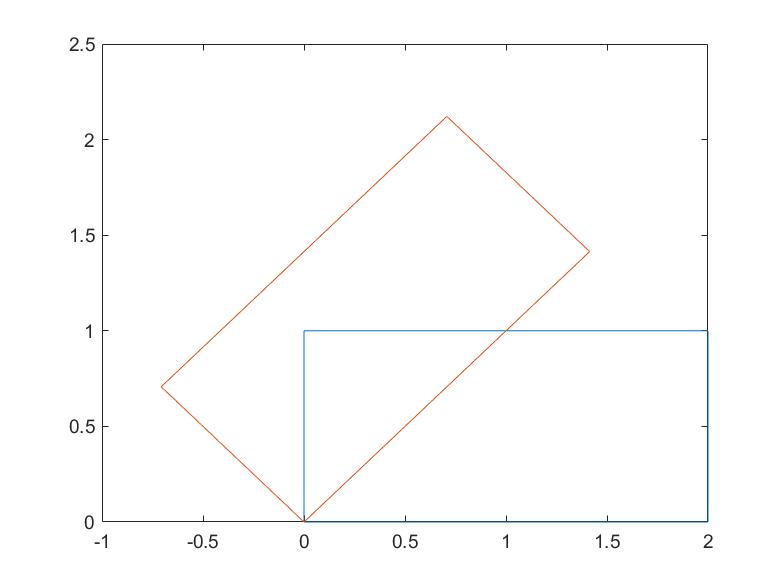
\includegraphics[width=.75\textwidth]{FacesNight2/figs/quizrot.jpg}
 \end{center}
What is the determinant of $\mathbf{M}$?

\item The orange shape is the result of applying a matrix $\mathbf{M}$ to the blue rectangle.
\begin{center}        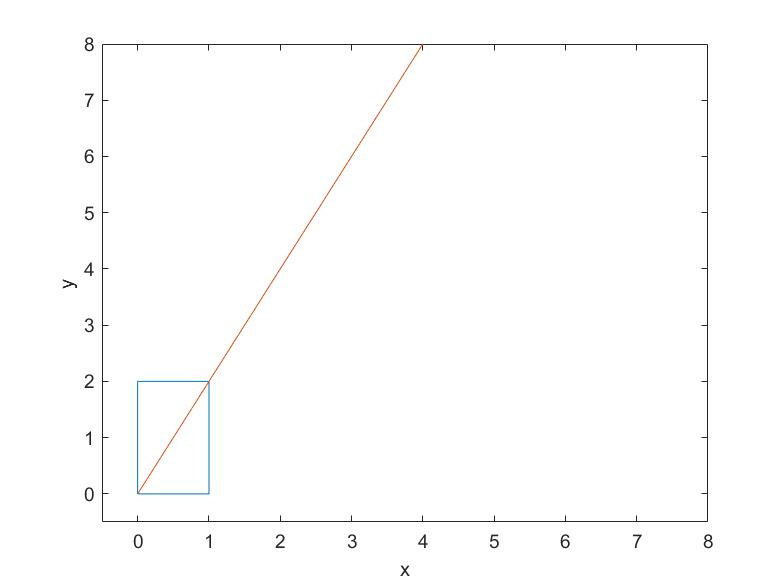
\includegraphics[width=.75\textwidth]{FacesDay2/figs/mat3.jpg}
 \end{center}
What is the determinant of $\mathbf{M}$?

\item The determinant is multiplicative, i.e, $\det(\mathbf{AB})=\det(\mathbf{A})\det(\mathbf{B})$. Let $\mathbf{M}$ be a matrix such that $\det(\mathbf{M})=\frac{1}{3}$. What's $\det(\mathbf{M}^{-1})$? (Hint: $\det(\mathbf{I})=1$.)

\item Let $R$ be a rectangle with area 1. Apply the scaling matrix $\mathbf{S} = \begin{bmatrix} s_1 & 0 \\ 0 & s_2 \end{bmatrix}.$ What is the area of $\mathbf{S}R$?

A. $\frac{s_1s_2}{2}$\\
B. 1\\
C. $s_1s_2$\\
D. $s_1 + s_2$\\

\item True or false: Any shearing matrix $\mathbf{S}$ and any rotation matrix $\mathbf{R}$ commute, i.e., $\mathbf{RS}=\mathbf{SR}$.

\end{enumerate}

\pagebreak
\shipoutAnswer

%\subsection{Determinants in the Context of Linear Equations}
%
%While the formula for the determinant of a $2\times 2$ matrix is quite straightforward, the procedure for computing the determinant of larger matrices is more difficult, but they are well known, and well documented.  Fortunately, MATLAB has the {\tt det} function which computes the determinant.
%\begin{enumerate}[resume]
%\item Consider the following matrix whose columns line in the same line.
%\begin{align}
%\mathbf{A} = \twobytwo{1}{2}{2}{4}
%\end{align}
%\begin{enumerate}
%\item What is det$(\A)$?
%\vfill
%\item Recall that you can interpret matrix-vector multiplication as taking a linear combination of the columns of the matrix. Write the following matrix-vector product as a sum of scaled versions of the columns of $\mathbf{A}$, and simplify by writing it as a scaled version of the first column of $\A$.
%    \begin{align}
% \A \twobyone{x_1}{x_2} = \v
%    \end{align}
%\item Your answer to the previous question should indicate that $\v$ can only be a vector that points in the direction $\twobyone{1}{2}$. In other words we can write $\v$ in terms of a some  number $q$ as follows
%    \begin{align}
%    \v = q \twobyone{1}{2}
%    \end{align}
%\item Now, combine your answers to the previous two parts to relate $x_1$ and $x_2$ to $q$, and show that there are multiple values of $x_1$ and $x_2$ which can satisfy this equation for a given $q$. As a result the equation
%    \begin{align}
%     \A \twobyone{x_1}{x_2} = \v
%    \end{align}
%    has multiple solutions, and so $\mathbf{A}$ cannot have a well defined inverse since (if we could take the inverse) $\A^{-1} \v$ could have multiple different values.
%
%\item With your table, discuss how the fact that the columns of $\A$ lying on the same line resulted in this property, and how this relates to the determinant.

%\end{enumerate}
%\end{enumerate}




%
%\section{The Big Picture, Redux [20 min]}
%\begin{enumerate}%[resume]
%\item With your team, write down the top ideas that you took away from today's class.

%\end{enumerate}


